%====================================================================
%                 B E S S E L   F U N C T I O N S
%====================================================================
\section{Bessel functions of the first kind}
The most basic idea about Bessel functions is that they are solutions to the Bessel differential equation.
%
%-----------------defn: bessel differential equation------------------
%
\begin{defn}The Bessel differential equation of order $\nu$ and argument $z$
  \begin{equation}\label{eq:bessel_differential}
      z^2 \frac{d^2 U}{dz^2} + z\frac{dU}{dz} + (z^2 - \nu^2)U = 0
  \end{equation}
for $\nu, z \in \bb{C}$.
\end{defn}\par
%
Applications in this project are concerned with Bessel functions of integer order only, so we replace $\nu \in \bb{C}$ with $n \in \bb{Z}$.
%------------------------defn: bessel function------------------------
%
\begin{defn}\label{defn:bessel_func}
Bessel functions are defined as follows,
  \begin{align*}
      J_n(z) = \sum^\infty_{m=0} \frac{
      (-1)^m (z/2)^{2m+n} }{
      m! (n+m)! }
  \end{align*}
\end{defn}
%
%------------propn: bessel function solves bessel equation------------
%
\begin{propn} Bessel functions of integer order solve the Bessel differential equation.
\end{propn}
\hl{This proof is new}
\begin{proof} The proof in \parencite{korenev02bessel_func} is conceptually similar to this but is given in much less detail.\par
  %
  We propose a solution to \eqref{eq:bessel_differential} in the form of a power series expansion
    \begin{equation*}
      U(z) = \sum_{m=0}^\infty c_m z^{m + \zeta}
    \end{equation*}
  where $c_0 \neq 0$.
  %
  This allows us to find expressions for the first and second derivatives,
    \begin{align*}
      U'(z) &= \sum_{m=0}^\infty c_m (m+\zeta) z^{m+\zeta-1}, \\
      U''(z) &= \sum_{m=0}^\infty c_m (m+\zeta)(m+\zeta-1) z^{m+\zeta-2}.
    \end{align*}
  Substituting these into \eqref{eq:bessel_differential},
    \begin{multline}\label{eq:bessel_proof_summation}
      z^2 \left\{ \sum_{m=0}^\infty c_m (m+\zeta)(m+\zeta-1) z^{m+\zeta-2}\right\} \\
        + z \left\{ \sum_{m=0}^\infty c_m (m+\zeta) z^{m+\zeta-1} \right\}
          + (z^2 - n^2) \left\{ \sum_{m=0}^\infty c_m z^{m + \zeta} \right\} = 0.
    \end{multline}
  We now want to collect all of the terms of order $z^{\zeta}$ and $z^{\zeta+1}$:
    \begin{multline*}
      c_0(\zeta)(\zeta-1)z^{\zeta} + c_1(\zeta+1)(\zeta)z^{\zeta+1} + \sum_{m=2}^\infty c_m (m+\zeta)(m+\zeta-1) z^{m+\zeta} \\
      + c_0(\zeta)z^{\zeta} + c_1(\zeta+1)(\zeta)z^{\zeta+1} + \sum_{m=2}^\infty c_m (m+\zeta) z^{m+\zeta} \\
      - n^2 c_0 z^{\zeta} - n^2 c_1 z^{\zeta+1} -n^2 \sum_{m=2}^\infty c_m z^{m + \zeta} + \sum_{m=0}^\infty c_m z^{m + \zeta+2} =0.
    \end{multline*}
  Collecting terms:
    \begin{multline*}
      z^{\zeta} \{ c_0(\zeta)(\zeta-1) +  c_0(\zeta) - n^2 c_0 \}
      + z^{\zeta+1} \{  c_1(\zeta+1)(\zeta) + c_1(\zeta+1)(\zeta) - n^2 c_1\} \\
      + \sum_{m=2}^\infty \left\{ c_m (m+\zeta)(m+\zeta-1) z^{m+\zeta} + c_m (m+\zeta) z^{m+\zeta} - n^2 c_m z^{m + \zeta} \right\}
      + \sum_{m=0}^\infty c_m z^{m + \zeta+2} =0.
    \end{multline*}
  Consider a change of variable for the last term: $m'=m+2$ where $m'$ is just a dummy variable. Then we have $m=0 \Rightarrow m'=2$, $m\rightarrow \infty \Rightarrow m' \rightarrow \infty$ , and $m'= m-2$. So we can rewrite the last term as a sum from $m'=2$,
    \begin{equation}
      \sum_{m'=2}^\infty c_{(m'-2)} z^{m' + \zeta} =0.
    \end{equation}
  Hence we are left with the following expression
    \begin{equation}
      z^{\zeta} c_0\{ \zeta^2 - n^2\} + z^{\zeta+1} c_1 \{ (\zeta+1)^2 -n^2\}
      + \sum_{m=2}^\infty \{ c_m [(m+\zeta)^2 -n^2] + c_{m-2} \}z^{m + \zeta} =0.
    \end{equation}
  This must be valid for all $z \in \bb{C}$, so all the coefficients of $z^{\zeta +m}$ must be equal to zero.
    \begin{gather}
      c_0\{ \zeta^2 - n^2\} = 0,\label{proof:bessel_c0} \\
      c_1 \{ (\zeta+1)^2 -n^2\} = 0 \label{proof:bessel_c1}\text{ and}\\
      c_m [(m+\zeta)^2 -n^2] + c_{m-2} = 0 \text{ for } m \in \bb{Z}^{\geq 2} \label{proof:bessel_cm}
    \end{gather}
  First consider \eqref{proof:bessel_c0}. We assumed at the start that $c_0\neq0$, so we must have that
      \begin{equation}
        \zeta = \pm n.
      \end{equation}
  Additionally, we can see there is a recursive relationship between all the coefficients $c_i$. Namely,
    \begin{align}
      c_m &= - \frac{c_{m-2}}{(m+\zeta^2)-n^2} = - \frac{c_{m-2}}{(m^2 +2m\zeta + \zeta^2 -n^2} \\
      &= - \frac{c_{m-2}}{m(m +2\zeta)} \text{ since } \zeta^2 = n^2.
    \end{align}
  Additionally, from \eqref{proof:bessel_cm} we can find the next terms in the sequence of coefficients for even $m$:
    \begin{align*}
      c_2 &= - \frac{c_0}{4(1+\zeta)}, \\
      c_4 &= - \frac{c_2}{8(2+\zeta)} = \frac{c_0}{4 \times 8 \times (1+\zeta) (2+\zeta)}, \\
      c_6 &= - \frac{c_3}{12(3+\zeta)} = - \frac{c_0}{4 \times 8 \times 12 \times (1+\zeta) (2+\zeta)(3+\zeta)}, ...
    \end{align*}
  Setting $\zeta = n$ we get the first partial solution for \eqref{eq:bessel_differential}
    \begin{align*}
      U_1(z) = c_0z^n \left\{
        1 - \frac{z^2}{4(1+n)} + \frac{z^4}{2!4^2(1+n) (2+n)} - \frac{z^6}{3!4^3(1+n)(2+n)(3+n)} + ...
        \right\},
    \end{align*}
  and setting $\zeta = -n$ we get a second partial solution
    \begin{align*}
      U_2(z) = c'_0z^{-n} \left\{
        1 - \frac{z^2}{4(1-n)} + \frac{z^4}{2!4^2(1-n) (2-n)} - \frac{z^6}{3!4^3(1-n)(2-n)(3-n)} + ...
        \right\}.
    \end{align*}
  For simplicity, the constants $c_0$ and $c'_0$ are set the following values.
  \begin{multicols}{2}
    \noindent
    \begin{align*}
      c_0 = \frac{1}{2^n \Gamma(1+n)}
    \end{align*}
    \begin{align*}
      c'_0 = \frac{1}{2^{-n} \Gamma(1-n)}
    \end{align*}
  \end{multicols}\par
  %
  Where $\Gamma$ is the Gamma function that extends the value of the factorial $n!$ to any complex number -- most importantly in this case to $n \in \bb{Z}_{< 0}$ \parencite{kuptsov11gammafunc}.\par
  %
  Consider the first solution. Note that for $n \in \bb{Z}^{\geq0}$, $\Gamma (n+1) =n!$.
  \begin{align*}
    U_1(z) &= \frac{1}{2^n n!} z^n \left\{
        1 - \frac{z^2}{2^2(1+n)} + \frac{z^4}{2!2^4(1+n) (2+n)} - \frac{z^6}{3!2^6(1+n)(2+n)(3+n)} + ...
        \right\},\\
      &= z^n \left\{
        1 - \frac{z^2}{2^{2+n} n!(1+n)} + \frac{z^4}{2!n! 2^{4+n} (1+n) (2+n)} - \frac{z^6}{3!n! 2^{6+n} (1+n) (2+n) (3+n)} + ...
        \right\}.
  \end{align*}
  We can see a pattern in the denominator,
  \begin{align*}
    \begin{array}{c|lll}
      \# &  \multicolumn{3}{c}{\text{denominator}}\\
      \hline
      0   &   1                                        \\
      1   &   2^{2+n} &   n!    &   (1+n)              \\
      2   &   2^{4+n} &   2!n!  &   (1+n) (2+n)        \\
      3   &   2^{6+n} &   3!n!  &   (1+n) (2+n) (3+n)
    \end{array}
  \end{align*}
  which can be expressed in terms of $\Gamma$ functions:
  \begin{align*}
    \Gamma(m+n+1) &= (m+n)! \\
      &= 1 \times 2 \times 3 \times ... \times n \times (n+1) \times ... \times (n+m) \\
      &= n! (n+1)(n+2)...(n+m).
  \end{align*}
  Note that this shows that the size of $n$ relative to $m$ is important. This will become relevant later. For $n<m$ we therefore have a general expression for the $m^{\text{th}}$ term of the series
  \begin{align*}
     \frac{(-1)^mz^{2m+n}}{2^{2m+n}m!\Gamma(m+n+1)}.
  \end{align*}
  Clearly this can also be done for the second solution. Hence we have an infinite summation expression for both sets of solutions. We call these $J_n$ and $J_{-n}$, which are in fact the functions defined in definition \ref{defn:bessel_func}.
  \begin{align*}
    J_n(z) = \left(\frac{z}{2}\right)^n \sum^\infty_{m=0} \frac{(-1)^m(z/2)^{2m}}{m!\Gamma(m+n+1)}, \\
    J_{-n}(z) = \left(\frac{z}{2}\right)^{-n} \sum^\infty_{m=0} \frac{(-1)^m(z/2)^{2m}}{m!\Gamma(m-n+1)}.
  \end{align*}
  \end{proof}

For $\nu$ not an integer, the collection of Bessel functions of different $\nu$ is linearly independent and is the general soltion to \ref{eq:bessel_differential}. However if $\nu = n \in \bb{Z}$ Bessel functions are linearly dependent. In particular, the following identity holds.

\begin{propn} \label{propn:bessel_int_order_identity} For $n \in \bb{Z}$,
  \begin{equation}
    J_n(z) = (-1)^n J_{-n}(z).
  \end{equation}

\end{propn}\par

Another useful result using Bessel functions of the first kind is the Jacobi expansion. This gives us a way to rewrite exponential functions as infinite sums of Bessel functions.

\begin{propn}\label{propn:jacobi_expansion}
\textbf{\emph{The Jacobi expansion.}}
    \[
    e ^{i \omega cos \varphi}
    = \sum^\infty_{n=-\infty} i^n J_n (\omega) e^{in\varphi}
    = \sum^\infty_{n=0} \epsilon_n i^n J_n(\omega) cos(n \varphi)
    \]
where $\epsilon_n$ is the Neumann factor, defined as follows.
    \begin{align*}
        \epsilon_n =\left\{
            \begin{array}{c l}
                 1 & n = 0 \\
                 2 & n \geq 1
            \end{array}\right.
    \end{align*}
\end{propn}
\begin{proof} TBD \parencite[$\S$2.5]{martin06scattering}
\end{proof}


%====================================================================
%                 bessel functions of the 2nd kind
%====================================================================
\section{Bessel functions of the second kind}

Bessel functions of the second kind, or Neumann functions are defined as a linear combination of $J_\nu$ and $J_{-\nu}$. These are useful because for $\nu = n$ an intger, Bessel equations are linearly dependent on each other. In fact, the following relationship holds \cite{korenev02bessel_func}
\[J_{-n}(z) = (-1)^n J_{n}(z)\].

We can define another solution to the Bessel differential equation, the Neumann function.

\begin{defn} Bessel functions of the second hand, or Neumann functions of order $\nu$ and argument $z$ are defined as follows.
  \[Y_\nu(z) = \frac{J_\nu(z) \cos (\nu \pi)- J_{-\nu}(z)}{\sin (\nu \pi)}\]
\end{defn}

However for integer $\nu=n$ this is undefined -- in fact the left hand side is $0/0$. In order to have a meaningful defintion of $Y_n$ we apply L'Hôpital's rule.

\begin{align*}
  Y_n(z) &= \lim_ {\nu \rightarrow n}\frac{J_\nu(z) \cos (\nu \pi)- J_{-\nu}(z)}{\sin (\nu \pi)} \\
      &= \lim_ {\nu \rightarrow n} \partialfrac{}{\nu} \frac{J_\nu(z) \cos (\nu \pi)- J_{-\nu}(z)}{\sin (\nu \pi)}
\end{align*}

%====================================================================
%               bessel functions of the 3rd kind
%====================================================================

\section{Bessel functions of the third kind}

%------------------------ defn: hankel -------------------------------
\begin{defn}\label{defn:hankel_func}
  Cylindrical functions of the third kind or Hankel functions, are linear combinations of Bessel functions of the first and second kind.
    \begin{align*}
        H^{(1)}_\nu(z) = J_\nu(z) + i Y_\nu(z)\\
        H^{(2)}_\nu(z) = J_\nu(z) - i Y_\nu(z)
    \end{align*}
  In particular, for $\nu = n \in \bb{Z}$,
    \begin{align*}
      H^{(1)}_\nu(z)
        &= \lim_{\nu \rightarrow n} \frac{J_{\nu}(z) - e^{-\nu\pi i} J_{-\nu}(z)}{i \sin(\nu \pi)} \\
      H^{(2)}_\nu(z)
        &= \lim_{\nu \rightarrow n} \frac{J_{\nu}(z) - e^{\nu\pi i} J_{-\nu}(z)}{- i \sin(\nu \pi)}
    \end{align*}
  from \cite{karmazina19cylinderfunc}.
\end{defn}

The following identities are well known \parencite{karmazina19cylinderfunc} and will be useful later on in the project.

\begin{propn}\label{propn:hankel_identities}
  \[ H^{(1)}_{-\nu}(z) = e^{i\nu\pi}H^{(1)}_{-\nu}(z)\]
  \[ H^{(2)}_{-\nu}(z) = e^{-i\nu\pi}H^{(2)}_{-\nu}(z) \]
\end{propn}
\begin{proof}
  Not given.
\end{proof}


%---------------------------------------------------------------------
%             LIMITS OF BESSEL FUNCTIONS at the origin
%---------------------------------------------------------------------
\section{Limits of Bessel functions at the origin}\label{ss:limits_of_bessel_functions}

%-------------------- bessel function at the origin ------------------
\begin{propn}\label{propn:bessel_at_origin}
  Bessel functions of the first kind of integer order are well defined at the origin. In particular,
  \begin{align}\label{propn:bessel_arg_zero}
      J_n(0) =\left\{
        \begin{array}{c l}
             1 & n = 0 \\
             0 & n \neq 0
        \end{array}\right.
  \end{align}
\end{propn}
\begin{proof}
  This is immediate from the definiton of Bessel functions (definition \ref{defn:bessel_func}).
    \begin{align*}
      J_n(x)
        &= \sum^\infty_{m=0} \frac{(-1)^m(x/2)^{n+2m}}{m! (n+m)!}\\
        &= \frac{(-1)^0(x/2)^{n}}{0!n!}         %m=0
          + \frac{(-1)^1(x/2)^{n+2}}{1!(n+1)!}  %m=1
          + \frac{(-1)^2(x/2)^{n+4}}{2!(n+2)!}  %m=2
          + \dotsb \\
        &= \left(\frac{x}{2}\right)^n
          \left[\frac{1}{n!}           %m=0
          - \frac{(x/2)^{2}}{(n+1)!}   %m=1
          + \frac{(x/2)^{4}}{2(n+2)!}  %m=2
          + \dotsb \right]\\
      \therefore
      J_0(x)
        &= 1
          - \frac{(x/2)^{2}}{2}
          + \frac{(x/2)^{4}}{12} + \dotsb
    \end{align*}
  Hence the function is well defined at $x=0$, and \ref{propn:bessel_arg_zero} holds for all $n \in \bb{Z}$.
\end{proof}\par

\begin{figure} \centering
  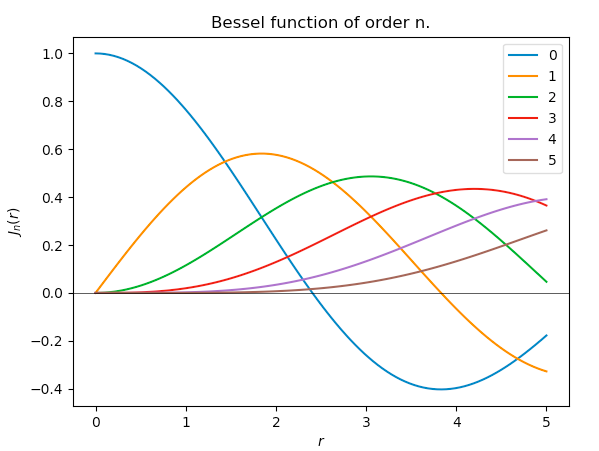
\includegraphics[width=8cm]{../figures/plot_bessel_int_order}
  \caption{Bessel functions of integer order.}\label{fig:bessel_int_problem}
\end{figure}

This result is clearly shown in \figref{fig:bessel_int_problem}.

%------------------- neumann functions at the origin -----------------
\begin{propn}\label{propn:neumann_singular_at_origin}
  Neumann functions are singular at the origin.
\end{propn}
%
\begin{proof}
  From the definition of Neumann functions (definition \ref{defn:neumann_func}) we know that for $n$ integer
    \begin{equation}
      Y_n(z=0) = \lim_{\nu \rightarrow n} \frac{J_\nu(0) \cos (\nu \pi) - J_{-\nu}(0)}{\sin (\nu \pi)}
    \end{equation}
  %
  First, consider the limit of the numerator as $\nu \rightarrow$ integer. Then
  %
    \begin{gather*}
      J_\nu(0) \rightarrow
        J_n(0) = \left\{
          \begin{array}{c l}
               1 & n = 0 \\
               0 & n \neq 0
          \end{array}\right. \text{ from proposition \ref{propn:bessel_at_origin},}\\
      J_{-\nu}(0) \rightarrow
        (-1)^nJ_n(0) = (-1)^n\left\{
          \begin{array}{c l}
               1 & n = 0 \\
               0 & n \neq 0
          \end{array}\right.
          = \left\{
            \begin{array}{c l}
                 1 & n = 0 \\
                 0 & n \neq 0
            \end{array}\right. \text{ from proposition \ref{propn:bessel_int_order_identity}.}\\
      \text{Hence } J_{\pm\nu}(0) \rightarrow
        \left\{
          \begin{array}{c l}
               1 & n = 0 \\
               0 & n \neq 0
          \end{array}\right.
    \end{gather*}
  Additionally,
    \begin{gather*}
      \cos(\nu\pi) \rightarrow (-1)^n.
    \end{gather*}
  We broady have two cases for the numerator, $n=0$ and $n\neq 0$.
    \begin{gather*}
      J_\nu(0)\cos(\nu\pi) - J_\nu(0) \rightarrow
      \left\{
        \begin{array}{c l}
             1\times1-1=0 & n = 0 \\
             0\times1-0=0 & n \neq 0
        \end{array}\right.
    \end{gather*}
  Now for the denominatory, clearly
    \begin{gather*}
      \sin(\nu\pi) \rightarrow 0.
    \end{gather*}
  This gives us the indeterminate limit $0/0$ at $x=0$ as $\nu \rightarrow$ integer.
\end{proof}
%
\begin{figure} \centering
  %
  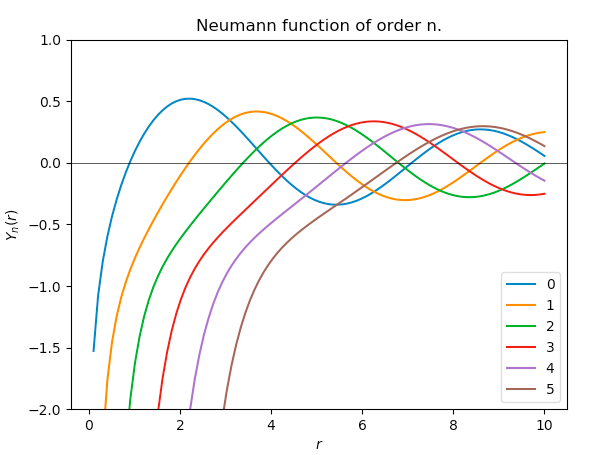
\includegraphics[width=8cm]{../figures/plot_neumann_int_order}
  \caption{Neumann functions of integer order.}\label{fig:neumann_int_problem}
  %
\end{figure}\par
%
\begin{propn}
  Hankel functions are singular at the origin.
\end{propn}
%
\begin{proof}
  This follows directly from the definition of Hankel functions for $n\in\bb{Z}$ (definition \ref{defn:hankel_func}), and can be proven in the same way as proposition \ref{propn:neumann_singular_at_origin}.
\end{proof}
%
\begin{figure} \centering
  %
  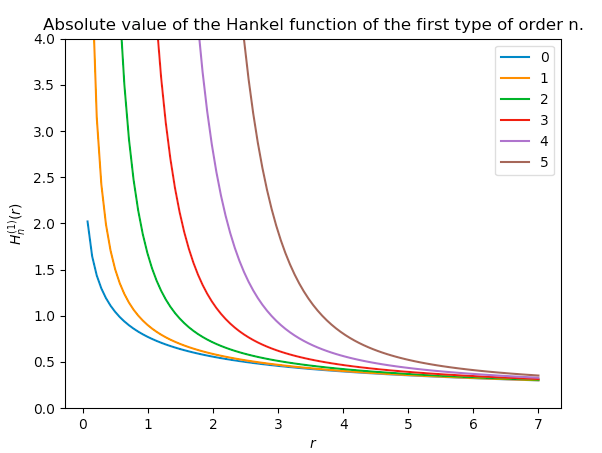
\includegraphics[width=8cm]{../figures/plot_hankel_int_order}
  \caption{Hankel functions of integer order.}\label{fig:neumann_int_problem}
  %
\end{figure}\par
